% ===============================================================================
% = LaTeX Beamer Template of the Signal Processing Group, Department of Informatics 
% = (c) 2016 Prof. Dr. Hannes Federrath, Uni Hamburg, Fachbereich Informatik
% = https://svs.informatik.uni-hamburg.de
% =
% = Weitgehend in Übereinstimmung mit dem Corporate Design 2016 der UHH:
% = https://www.uni-hamburg.de/beschaeftigtenportal/services/oeffentlichkeitsarbeit/corporate-design.html
% = 
% ===============================================================================
%
\documentclass[10pt]{beamer} 
% Option t              Place text of slides at the (vertical) top of the slides.
% Option handout        Ein PDF ohne Pausen und Overlayeffekte erzeugen.
% Option aspectratio=43 169 => 16:9, 1610 => 16:10, 43 => 4:3

% Use SP theme and include all necessary packages
% The following options can be specified:
%   okular          -   embed media suitable for Okular (works with .wav)
%   acrobat         -   embed media suitable for Adobe Reader (works with .mp3) 
%   externalviewer  -   embed media such that an external player is opened
%   footauthor      -   display short author names in foot line
%   foottitle       -   display short title in foot line
\usepackage[]{beamersp2017}

\addbibresource{bibliography/Bibliography.bib}

\usepackage{lipsum}
\usepackage{listings}
%\tikzexternalize[optimize=false,prefix=compiledFigs/]
% =============================
% = Ab hier Inhalte ändern... 
% =============================

\title[This is the short title]{Real-Time Automatic Gain Control for Singing Voice Applications}
%\subtitle{Real}
\author[Short Name]{Nils Heine}
\institute[Uni Hamburg]{University of Hamburg\\ Department of Informatics}
\date{\today}

\tikzexternalize[prefix=./compiledFigs/] %speeds up compilation

\begin{document}

\begin{frame}[plain]
    % Die Titelseite erscheint nach erneutem Übersetzen korrekt.
    \maketitle
\end{frame}

\begin{frame}{Outline}
    % Die Gliederung erscheit nach erneutem Übersetzen korrekt.
    \tableofcontents
\end{frame}

\section{Motivation}

\sectionPage{Motivation}

%\graphicspath{ {/Users/Matze/Documents/Bachelor\ Arbeit/Vortrag/SPBeamer/images/} }

\begin{frame}[c]{Motivation}{}
	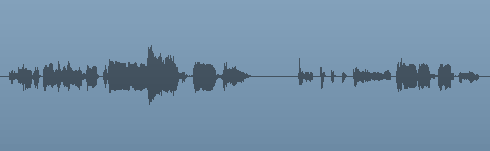
\includegraphics[scale=0.6]{images/wave}
	\centering
\end{frame}

\begin{frame}[c]{Motivation}{}
	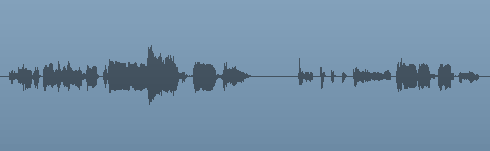
\includegraphics[scale=0.6]{images/wave}
	\centering
	\\
	\begin{itemize}
		\item compressor to fast
	\end{itemize}
\end{frame}

\begin{frame}[c]{Motivation}{}
	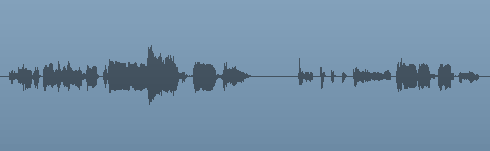
\includegraphics[scale=0.6]{images/wave}
	\centering
	\\
	\begin{itemize}
		\item compressor to fast \inlineitem factor in human perception
	\end{itemize}
\end{frame}

\begin{frame}[c]{Motivation}{}
	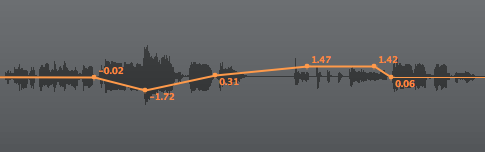
\includegraphics[scale=0.6]{images/auto}
	\centering
	\\
	\begin{itemize}
		\item compressor to fast \inlineitem factor in human perception \inlineitem save time
	\end{itemize}
\end{frame}

\begin{frame}[c]{Dummy UI}{}
	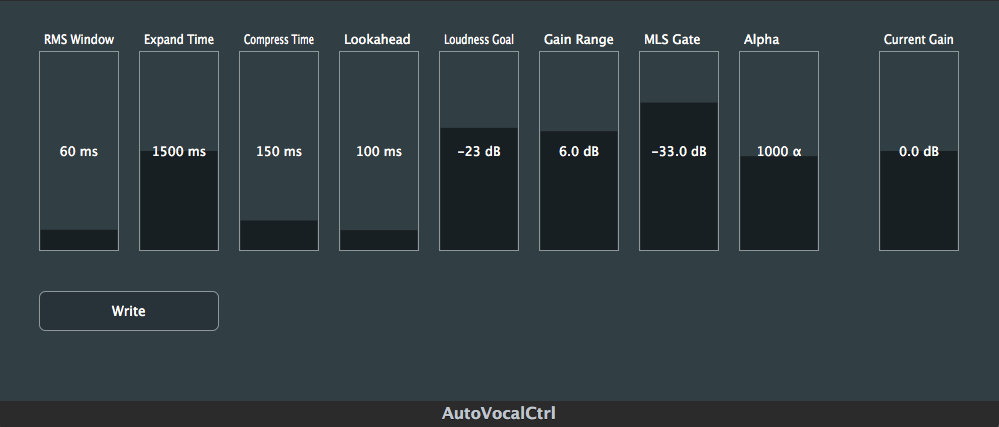
\includegraphics[scale=0.31]{images/plugin}
	\centering
\end{frame}


%JUCE FRAMEWORK BLA BLA

\section{Algorithm}

\sectionPage{Algorithm}

\begin{frame}[c]{Algorithm}{}
    \begin{enumerate}
        \setcounter{enumi}{1}
        \item Algorithm
            \begin{enumerate}
                \item Filter
                \item RMS
            		\begin{enumerate}
                		\item Time Coefficients     
            		\end{enumerate}
                \item Gate
                \item Gain
            		\begin{enumerate}
					\item Loudness Goal Adaption  
					\item Write Automation  
            		\end{enumerate}
                \item Lookahead
            \end{enumerate}
    \end{enumerate}
\end{frame}

\begin{frame}[c]{Algorithm: Filter}{}
	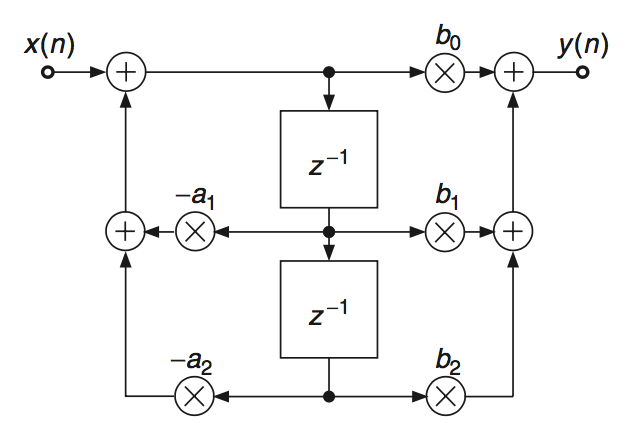
\includegraphics[scale=0.3]{images/biquat}
	\centering
    \footfullcite{Figure from DAFX: Digital Audio Effects by Udo Zoelzer}

    \printbibliography%
\end{frame}

\begin{frame}[c]{Algorithm: Filter}{}
	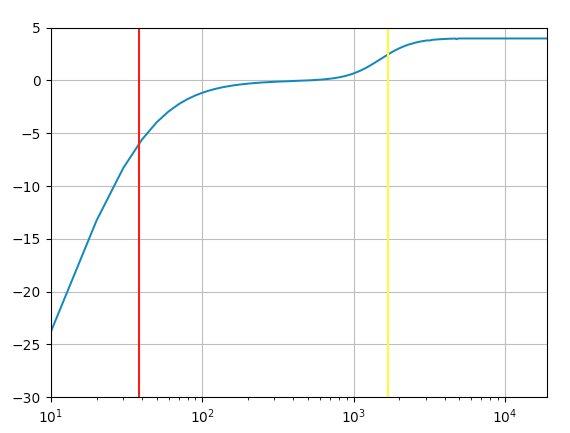
\includegraphics[scale=0.3]{images/filter}
	\centering\\
	\bigskip
    \begin{itemize}
    		\item lowcut (38 Hz), highshelf (1681 Hz) \footfullcite{from Recommendation ITU-R BS.1770-4}
    \end{itemize}

    \printbibliography%
\end{frame}

\begin{frame}[fragile]{Algorithm: RMS}{}
	Root Mean Square (RMS):
	\lstset{language=C++}
	\begin{lstlisting}[basicstyle=\tiny]
void AutoVocalCtrlAudioProcessor::updateRMS(int channel)
{
    rms[channel] = (1. - rmsCo) * rms[channel] +
                   rmsCo * (filterSample[channel] * filterSample[channel]);
}
	\end{lstlisting}
	\footfullcite{Based on Book: Digital Audio Signal Processing by Udo Zoelzer}\\
	\bigskip
	Time Constants:
	\begin{lstlisting}[basicstyle=\tiny]
float AutoVocalCtrlAudioProcessor::getTimeConstant(float ms)
{
    if (ms > 0.f)
        return 1.f - exp(-2.2*(1./currentSampleRate)/(ms/1000.));
    else
        return 1.f;
}
	\end{lstlisting}
	\footnotemark[2]
	
    \printbibliography%
\end{frame}

\begin{frame}[c]{Algorithm: Gate}{}
	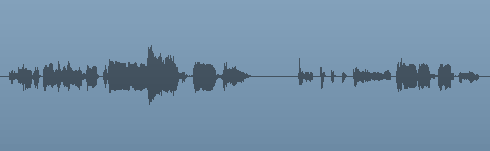
\includegraphics[scale=0.6]{images/wave}
	\centering
\end{frame}

\begin{frame}[fragile]{Algorithm: Gain}{}
	\lstset{language=C++}
	\begin{lstlisting}[basicstyle=\tiny]
void AutoVocalCtrlAudioProcessor::updateGain(int channel)
{
    const double g = *loudnessGoal - mls[channel];
    const double co = g < gain[channel] ? compressTCo:expandTCo;
    gain[channel] = clipRange.clipValue((1 - co) * gain[channel] + co * g);
    updateAutomation();
    ...
}
	\end{lstlisting}
\end{frame}

\begin{frame}[fragile]{Algorithm: Gain: Loudness Goal Adaption}{}
	\lstset{language=C++}
	\begin{lstlisting}[basicstyle=\tiny]
void AutoVocalCtrlAudioProcessor::updateGain(int channel)
{
    ...
    alphaGain[channel] = (1 - alphaCo) * alphaGain[channel] + alphaCo * gain[channel];
    if (channel == getTotalNumInputChannels() - 1)
    {
        ...
        updateLoudnessGoal();
    }
}
	\end{lstlisting}
\end{frame}

\begin{frame}[fragile]{Algorithm: Gain: Write Automation}{}
	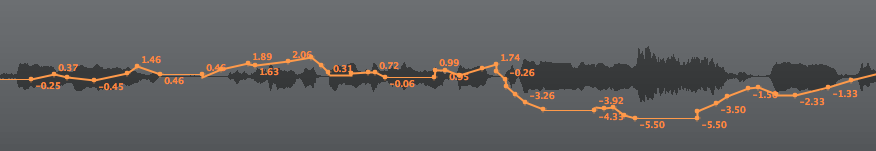
\includegraphics[scale=0.365]{images/automation}
	\centering
\end{frame}

\begin{frame}[c]{Algorithm: Lookahead}{per ringbuffer}
	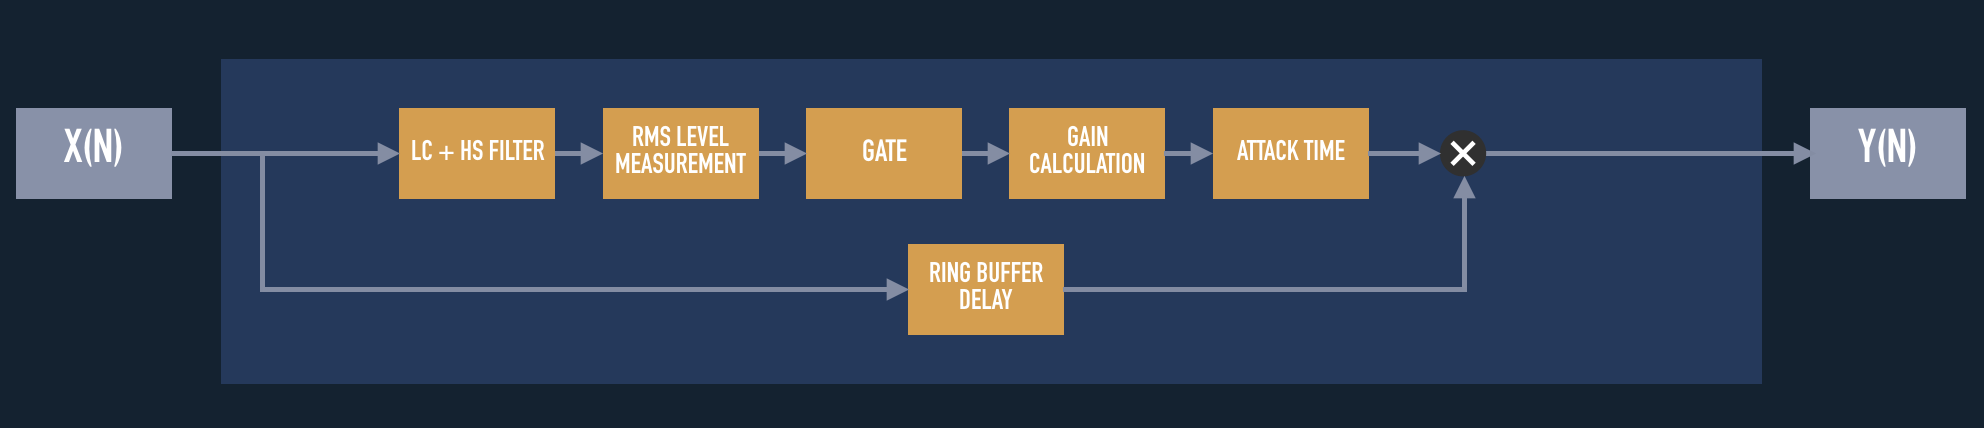
\includegraphics[scale=0.32]{images/lookahead}
	\centering
	\\
\end{frame}

\section{Optimization}

\sectionPage{Optimization}

\begin{frame}[fragile]{Optimization}{}
	\lstset{language=Python}
	\begin{lstlisting}[basicstyle=\tiny]
...
res = optmze.brute(compareGainCurve, bnds, full_output=True, finish=optmze.fmin)
...
res = optmze.minimize(compareGainCurve, x0, bounds=bnds, options={'disp': True, 'eps': 0.5})
...
x1 = np.array([-28.22, 5.65, 110.14, 2044.41, -33.94, 0.])
...
	\end{lstlisting}
\end{frame}

\begin{frame}[c]{Optimization: Results}{}
	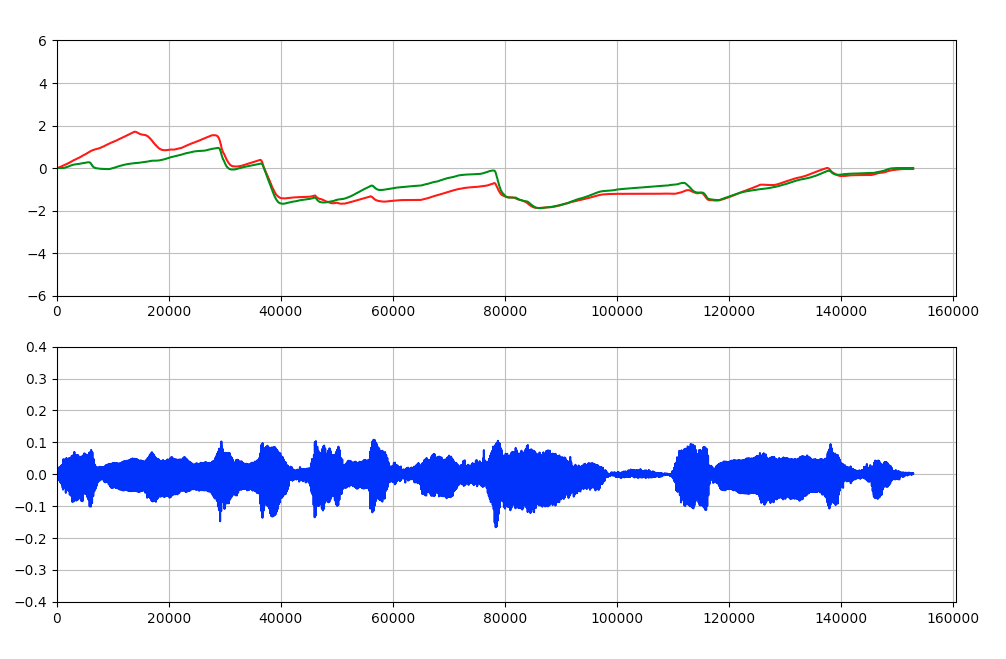
\includegraphics[scale=0.32]{images/optiG}
	\centering
\end{frame}


\chapter{Results}
\label{chapter:results}

The realisation of the objective could be achieved with a satisfactory result. During the process of development the JUCE Framework emphasises as a good choice by supporting with basic but solid functionality for an audio plug-in which would have been very time-consuming to build up from scratch.\\
With the first prototype version it was already possible to obtain favourable results (reasonable parameter settings implied). Nevertheless it still had some unfavorable problems and unfinished design decisions. The comparison to “Vocal Rider” approved the functionality of the prototype but also pointed out the differences between the two approaches of the plug-ins. Despite the differences the comparison resulted in ideas for further improvements of the study plug-in.\\
In retrospective view quite a lot improvements enhanced the early prototype. The additions with most influence on the plug-ins performance where the extra idle time for ignoring small breathing or rhythmic gaps between vocal signals, the ability to draw gain automations into the DAW, the side chain feature and the automatic detection of parameters.\\
The side chain feature validated its use in the according hearing test where its advantages for the plug-in where observable as well as the outcome of a plug-in with this feature enabled getting quite close to the optimal reference (which performed the gain adaption with oracle knowledge).\\

\section{Future Improvements}

The study plug-in meets the requirement of the objective but it could still be improved.\\
For example, parameter detection is an optional feature which could be useful to set the plug-in correctly, especially at first interactions of a user but as described in the corresponding chapter \ref{chapter:improvements}.2 and \ref{chapter:improvements}.3, it is only able to calculate ‘online’ during playback of the song. An offline calculation is not implemented yet which would be significantly faster. As one purpose of the plug-in is to save time for the mixing engineer, it would be great to enhance the feature with offline calculations in future development. When the offline calculation is possible it would be able to measure the perceived signal level by using the loudness algorithm\cite{ITUalgo} which may improve the plug-in’s outcome.\\
An other option of a reasonable future improvement would be to extend its scope of application. Currently it is designed to work with vocal signals but other recordings may show similar problems e.g. recordings of the bass guitar. Therefore it would be useful to have the opportunity to chose between different presets for the main constants of the plug-in’s calculation, fitting the different signals.\\
Additional to possible algorithmic improvements the plug-in could be improved by further testing for increased stability and correctness of the results.\\

\section{Conclusion}

A plug-in for decreasement of long term dynamics was developed. During the work on this study the plug-in’s prototype frequently changes and additional improvements in terms of features, algorithms and parameters were included.\\
It certainly might get further improvements in different parts but in final conclusion the study resulted in a plug-in mature enough to fulfil its intended task in daily production, and even some features more.\\





\section{Future Implementations}

\sectionPage{Future Implementations}

\begin{frame}[c]{Future Implementations}{}
    \begin{itemize}
    	\item side chain backtrack
    	\item offline loudness goal calculation
    	\item set parameters \filledrightarrow[uhhblue] simplify UI
    	\item improve writing of automation
    	\item idle time?
    	\item wet / dry?
    \end{itemize}
\end{frame}


%\section{Predefined Colors}

\sectionPage{Predefined Colors}

\begin{frame}[c, fragile]{Colors}
    \begin{itemize}
        \item Predefined colors are
            \begin{itemize}
                \item {\color{uhhblue} \verb|uhhblue rgb(0,156,209)|}
                \item {\color{uhhgreen} \verb|uhhgreen rgb(66,178,60)|}
                \item {\color{uhhred} \verb|uhhred rgb(226,0,26)|}
                \item {\color{uhhblack} \verb|uhhblack rgb(0,0,0)|}
                \item {\color{uhhstone} \verb|uhhstone rgb(59,81,91)|}
            \end{itemize}
    \end{itemize}
\end{frame}


%\section{Itemize and Enumerate}

\sectionPage{Itemize and Enumerate}

\begin{frame}[c, fragile]{Itemize and Enumerate}{Itemize Environment}
    \begin{itemize}
        \item First level
            \begin{itemize}
                \item Second Level
                    \begin{itemize}
                        \item Third level
                    \end{itemize}
            \end{itemize}
        \item[\cmark] This is good (\verb|\cmark|)
        \item[\xmark] This is bad (\verb|\xmark|)
        \item[\filledrightarrow] This is follows from the upper points (\verb|\filledrightarrow|)
            \begin{itemize}
                \item This follows \filledrightarrow[uhhblue]~inline (\verb|\filledrightarrow[uhhblue]|)
            \end{itemize}
    \end{itemize} 
\end{frame}

\begin{frame}[c]{Itemize and Enumerate}{Enumerate Environment}
    \begin{enumerate}
        \item First level
            \begin{enumerate}
                \item Second level
                    \begin{enumerate}
                        \item Third level
                    \end{enumerate}
            \end{enumerate}
    \end{enumerate}
\end{frame}


%\section{Blocks}

\sectionPage{Blocks}

\begin{frame}[c]{Blocks}{Block Demonstration}
    \begin{block}{This is the Block Title}
        \lipsum[1]%
    \end{block}
    
\end{frame}


%\section{Citations}

\sectionPage{Citations}

\begin{frame}[c]{Citations\footfullcite{gerkmann_bayesian_2014}}
    \begin{itemize}
        \item Another citation\footfullcite{breithaupt_parameterized_2008}
        \item Always cite Timo\footfullcite{gerkmann_improved_2008}
        \item Bibliography can be included on any slide
    \end{itemize}

    \printbibliography%
\end{frame}


%\section{Audio}

\sectionPage{Audio}

\begin{frame}[c, fragile]{Audio}
    \begin{itemize}
        \item Play some sound: \spaudio{audioexamples/timit.mp3} 
        \item Realized using \verb|\spaudio{audioexamples/timit.mp3}|
        \item switch for Acrobat Reader in beamersp2017.sty \verb|\usepackage[acrobat]{beamersp2017}|
    \end{itemize}
\end{frame}


%\section{TikZ Extensions}

\sectionPage{TikZ Extensions}

\begin{frame}[c]{TikZ Extensions}{Overlay Effects in TikZ Images}
    \centering
    \begin{tikzpicture}[thick]
        \draw[visible on=<1->, onslide=<5->uhhred, -latex] (0, 0) -- (1, 0);
        \draw[visible on=<2->, onslide=<6->uhhgreen, -latex] (1, 0) -- (1, 1);
        \draw[visible on=<3->, onslide=<7->uhhblue, -latex] (1, 1) -- (0, 1);
        \draw[visible on=<4->, onslide=<8->uhhstone, -latex] (0, 1) -- (0, 0);
    \end{tikzpicture}
    \vspace{2ex}
    \begin{itemize}
        \item<1-> \texttt{visible on=<num-num>}: make node edge visible on that slide
        \item<5-> \texttt{onslide=\{<num-num>style\}}: apply style on given slides
    \end{itemize}
\end{frame}

\begin{frame}[c]{TikZ Extensions}{Standalone Legends}
    \centering
    \begin{tikzpicture}
        \begin{customlegend}[%
                legend entries={%
                    Entry 1,
                    Entry 2,
                    Entry 3 with comments,
                    Entry 4,
                },
                legend columns={2},
                legend cell align={left},
                legend style={draw=none},
            ]
            \addlegendimage{thick, uhhblue};
            \addlegendimage{area legend, thick, draw=none, fill=uhhred};
            \addlegendimage{surf, thick};
            \addlegendimage{dashed, uhhstone, mark=*}
        \end{customlegend}
    \end{tikzpicture}
    \vspace{2ex}
    \begin{itemize}
        \item Custom legends using \texttt{customlegend} environment
    \end{itemize}
\end{frame}

\begin{frame}[c]{TikZ Extensions}{A Sine in TikZ}
    \centering
    \begin{tikzpicture}
        \begin{axis}[
                scale only axis,
                axis x line=middle,
                axis y line=middle,
                xlabel={$t$},
                ylabel={$x_a(t) = A \cos(2\pi f - \theta)$},
                ymin=-2,
                ymax=2,
                width=6cm,
                height=4cm,
                xtick={0},
                ytick={1},
                yticklabels={$A$},
                yticklabel style={right},
            ]
            \addplot[blue, mark=none, domain=-4:4, samples=500, name path=cos] {cos(deg(2*x + 1))};

            \path[name path=yaxis] (axis cs:0, -2) -- (axis cs:0, 2);

            \path [name intersections={of=cos and yaxis,by=E}];

            \node[fill=blue, circle, inner sep=1pt, pin=30:$A\cos(\theta)$] at(E) {};

            \draw (axis cs:-2.07, -0.75) -- (axis cs:-2.07, -1.25);
            \draw (axis cs:1.07, -0.75) -- (axis cs:1.07, -1.25);
            \draw[latex-latex] (axis cs:-2.07, -1.25) -- node[below] {$T = 1/f$} (axis cs:1.07, -1.25);
        \end{axis}
    \end{tikzpicture}
    \vspace{2ex}
    \begin{itemize}
        \item Demo on how to plot a sine in TikZ
    \end{itemize}
\end{frame}

\begin{frame}[c]{TikZ Extensions}{An STFT Framework in TikZ}
    \centering
    \pgfplotsset{ax_stft/.style={%
	scale only axis,
	axis on top,
	xtick={\empty},
	ytick={\empty},
	xticklabels={\empty},
	yticklabels={\empty},
	width=0.3\textwidth,
	height=7ex,
	axis lines=middle,
	enlarge x limits=0.1,
	enlarge y limits=0.1,
	every axis x label/.style={at={(current axis.right of origin)},anchor=south west},
	every axis y label/.style={at={(current axis.above origin)},anchor=south}
	}
}%
%
\begin{tikzpicture}[
	box/.style={draw, fill=uhhblue, text=white, text width=5.5em, minimum height=4.5em, align={center}},
	frame annotation/.style={text=black, font=\footnotesize, above},
	frame boundaries/.style={fill=white, font=\footnotesize, inner sep=1pt}
]

\begin{axis}[
	ax_stft,
	xlabel={time},
	ylabel={noisy speech},
	name={noisy},
]
	\addplot[solid, uhhblue] table[x=sample, y=noisy] {data/stft.tsv};
\end{axis}

\begin{axis}[
	ax_stft,
	xlabel={time},
	at={($(noisy.south) - (0,1ex)$)},
	anchor=north,
	clip=false,
]
	\addplot[densely dotted, uhhblue] table[x=sample, y=win1] {data/stft.tsv} node[pos=0.25, frame annotation] {$\ell - 2$};
	\addplot[dashed, uhhblue] table[x=sample, y=win2] {data/stft.tsv} node[pos=0.5, frame annotation] {$\ell - 1$};
	\addplot[solid, uhhblue] table[x=sample, y=win3] {data/stft.tsv} node[pos=0.75, frame annotation] {$\ell$};

	\coordinate (noisy frame center) at(axis cs: -256, 0);
	\coordinate (noisy frame end) at(axis cs: -511, 0);
	\coordinate (noisy frame start) at(axis cs: 0, 0);
\end{axis}

\node[box, below=6ex of noisy frame center] (dft) {DFT};
\node[box, right=of dft, onslide=<2->{fill=uhhgreen}] (enhancement) {speech\\ enhancement};
\node[box, right=of enhancement] (idft) {IDFT};

\begin{axis}[
	ax_stft,
	xlabel={time},
	ylabel={enhanced speech},
	name={clean},
	at={($(idft.east |- noisy) - (2ex,0)$)},
	anchor=origin,
]
	\addplot[solid, uhhblue] table[x=sample, y=clean] {data/stft.tsv};
\end{axis}

\begin{axis}[
	ax_stft,
	xlabel={time},
	at={($(clean.south) - (0,1ex)$)},
	anchor=north,
	clip=false,
]
	\addplot[densely dotted, uhhblue] table[x=sample, y=win1] {data/stft.tsv} node[pos=0.25, frame annotation] {$\ell - 2$};
	\addplot[dashed, uhhblue] table[x=sample, y=win2] {data/stft.tsv} node[pos=0.5, frame annotation] {$\ell - 1$};
	\addplot[solid, uhhblue] table[x=sample, y=win3] {data/stft.tsv} node[pos=0.75, frame annotation] {$\ell$};

	\coordinate (clean frame center) at(axis cs: -256, 0);
	\coordinate (clean frame end) at(axis cs: -511, 0);
	\coordinate (clean frame start) at(axis cs: 0, 0);
\end{axis}

\draw[-] (noisy frame end) -- node[frame boundaries] {$K - 1$} (noisy frame end |- dft.north);
\draw[-] (noisy frame start) -- node[frame boundaries] {$0$} (noisy frame start |- dft.north);
\draw[-latex] (noisy frame center) -- (noisy frame center |- dft.north);

\draw[-] ($(dft.east) - (0, 4ex)$) -- node[frame boundaries] {$K - 1$} ($(enhancement.west) - (0, 4ex)$);
\draw[-] ($(dft.east) + (0, 4ex)$) -- node[frame boundaries] {$0$} ($(enhancement.west) + (0, 4ex)$);
\draw[-latex] (dft) -- node[yshift=1.2ex, font=\small] {$Y_{k, \ell}$} (enhancement);

\draw[-] ($(enhancement.east) - (0, 4ex)$) -- node[frame boundaries] {$K - 1$} ($(idft.west) - (0, 4ex)$);
\draw[-] ($(enhancement.east) + (0, 4ex)$) -- node[frame boundaries] {$0$} ($(idft.west) + (0, 4ex)$);
\draw[-latex] (enhancement) -- node[yshift=1.2ex, font=\small] {$\hat{S}_{k, \ell}$} (idft);

\draw[-] (idft.north -| clean frame end) -- node[frame boundaries] {$K - 1$} (clean frame end);
\draw[-] (idft.north -| clean frame start) -- node[frame boundaries] {$0$} (clean frame start);
\draw[-latex] (idft.north -| clean frame center) -- (clean frame center);

\node at($(noisy.north) + (-4em, 2em)$) (spk noisy) {
\includegraphics[width=1.5em]{graphics/PersonRed.pdf}};
\node at($(noisy.north) + (0em, 2.5em)$) (noise) {
\includegraphics[width=1.5em]{graphics/Monkey.pdf}};

\draw[red, decoration={expanding waves, angle=30, segment length=0.5ex}, decorate] (spk noisy) -- (noisy);
\draw[brown, decoration={expanding waves, angle=30, segment length=0.5ex}, decorate] (noise) -- (noisy);

\node at($(clean.north) + (-4em, 2em)$) (spk clean) {
\includegraphics[width=1.5em]{graphics/PersonRed.pdf}};

\draw[red, decoration={expanding waves, angle=30, segment length=0.5ex}, decorate] (spk clean) -- (clean);

\end{tikzpicture}%
%

\end{frame}

\begin{frame}[c, fragile]{TikZ Extensions}{An STFT Framework in TikZ}
    \begin{itemize}
        \item Some notes on the STFT framework picture
        \item It requires the following files
            \begin{itemize}
                \item \verb|data/STFT.tex|
                \item \verb|graphics/PersonRed.pdf|
                \item \verb|graphics/Monkey.pdf|
            \end{itemize}
        \item Changing the folders of these files requires editing of the graphic itself
        \item The graphic itself is given in \verb|graphics/STFT.tex|
    \end{itemize}
\end{frame}

% \begin{frame}[c]{TikZ Extensions}{Image plots}
%     \centering
%     \begin{tikzpicture}[]
%         \begin{groupplot}[
%                 group style={%
%                     group size={2 by 2},
%                     xlabels at=edge bottom,
%                     ylabels at=edge left,
%                     horizontal sep=2.5cm,
%                 },
%                 axis on top,
%                 scale only axis,
%                 ymin=0,
%                 ymax=4,
%                 xmin=1.75,
%                 xmax=3.5,
%                 colormap name=viridis,
%                 xlabel={$t~/~\text{s}$},
%                 ylabel={$f~/~\text{kHz}$},
%                 width=0.3\linewidth,
%                 height=2.5cm,
%                 colorbar,
%                 colorbar style={width=2ex, xshift=-2ex},
%                 title style={anchor=south, at={(0.5, 0.9)}},
%             ]
%             \nextgroupplot
%             \imagesc{data/spectrogram_noisy.tsv}
% 
%             % Use different color range
%             \nextgroupplot[
%                 title={Different color range},
%                 point meta min=-30,
%                 colormap name=hot2,
%                 point meta max=0]
%             \imagesc{data/spectrogram_noisy.tsv}
%             \node[draw, fill=white, anchor=north west, font=\footnotesize] at (rel axis cs:0, 0.99) {colormap name=hot2};
% 
%             % Show different excerpt
%             \nextgroupplot[
%                 title={Other excerpt},
%                 point meta min=-30,
%                 point meta max=0,
%                 colormap name=parula,
%                 xmin=2.75,
%                 xmax=4.5,
%                 ymin=0,
%                 ymax=8]
%             \imagesc{data/spectrogram_noisy.tsv}
%             \node[draw, fill=white, anchor=north west, font=\footnotesize] at (rel axis cs:0, 0.99) {colormap name=parula};
% 
%             % Use custom defined colormap (it's intentionally ugly)
%             \nextgroupplot[
%                 title={Custom Colormap},
%                 colormap name=temp, 
%                 point meta min=-30,
%                 point meta max=10,
%                 xmin=3.5,
%                 xmax=5.5]
%             \imagesc{data/spectrogram_noisy.tsv}
%             \node[draw, fill=white, anchor=north west, font=\footnotesize] at (rel axis cs:0, 0.99) {colormap name=temp};
%         \end{groupplot}
%     \end{tikzpicture}
% \end{frame}


\begin{frame}{Outline}
    % Die Gliederung erscheit nach erneutem Übersetzen korrekt.
    \tableofcontents
\end{frame}

\end{document}
